\documentclass{ctexbeamer}
\usepackage{graphicx}
\usepackage{xcolor}
\usepackage{amssymb}
\usepackage{amsfonts}
\usepackage{pifont}
\usepackage{bm}
\usepackage{subcaption}
\def\E{\mathbb{E}}
\def\R{\mathbb{R}}
\DeclareMathOperator{\Vol}{Vol}
\newif\ifbeamer
\beamertrue

%further improvement
%background intro added Chen Chuan's work
%simulation add hierarchical method
%find suitable dataset to apply info-clustering
%Yang Li's suggestion: compared with other clustering method, the threshold is the same or not
%early stopping technique, complexity from n -> log(n)
\title{The Canonical Ensemble}
%\author{Feng Zhao}
\date{\today}
\begin{document}
\begin{frame}
	\titlepage
\end{frame}
\begin{frame}{Outline}
    \tableofcontents
\end{frame}
\section{3.1 Equilibrium between 
a system and a heat reservoir
}

\begin{frame}
\frametitle{正则系综}
\begin{itemize}
    \item 自变量:$N,V,T$
    \item 分布函数:$P_r \propto \exp(-\beta E_r)$
\end{itemize}

\end{frame}
\section{3.2 A system in the canonical ensemble
}
\begin{frame}
    \frametitle{正则系综概率分布的推导}
    \begin{enumerate}
        \item 最可几方法:拉格朗日乘子法求带约束的优化问题的最大值
        \item 平均值方法
    \end{enumerate}
    
    \end{frame}
\section{3.3 Physical significance of the various statistical quantities in
the canonical ensemble}
\begin{frame}{3.3 正则系综的热力学公式}
    \begin{enumerate}
        \item 配分函数:$Q_N(V,T) = \sum_{r} \exp(- \beta E_r)$
        \item 内能公式: $U=-\frac{\partial \ln Q_N(V,T)}{\partial \beta}$
        \item 熵公式: $S=-k\langle \ln P_r \rangle$,与信息论的熵的联系
    \end{enumerate}
\end{frame}
\section{3.5 The classical systems}
\begin{frame}{3.5 由正则系综推导单原子理想气体热力学公式}
    \begin{enumerate}
        \item 配分函数:$Q_N(V,T) = \frac{1}{N!} \left[ \frac{V}{h^3}(2\pi mkT)^{3/2} \right]^N$
        \item 内能公式: $U=-\frac{\partial \ln Q_N(V,T)}{\partial \beta}=\frac{3}{2}NkT$
        \item 熵公式: $S=-\frac{ \partial (kT \ln Q_N(V,T))}
        { \partial T}$
    \end{enumerate}
\end{frame}
\section{3.6 Energy fluctuation in the canonical ensemble: correspondence with the microcanonical ensemble}
\begin{frame}{3.6 正则系综的能量涨落}
    \begin{itemize}
        \item 在平均值附近的能量涨落很小
        \item 正则系综与微正则系综导出相同的热力学公式
    \end{itemize}
\end{frame}
\section{Two theorems -- the "equipartition" and the "virial"}
\begin{frame}{能量均分定理}
\begin{itemize}
    \item $\langle H \rangle = \frac{1}{2} fkT$
    \item $f$: 系统的自由度
\end{itemize}
\end{frame}
\section{A system of harmonic oscillators}
\begin{frame}{经典谐振子与薛定谔振子}
    \begin{itemize}
        \item 经典谐振子配分函数可通过状态空间积分的方法得到
        \item 薛定谔振子配分函数通过等比极数求和得到
        \item 在温度很低时,两者有明显区别;高温时等价
    \end{itemize}
    \begin{center}
    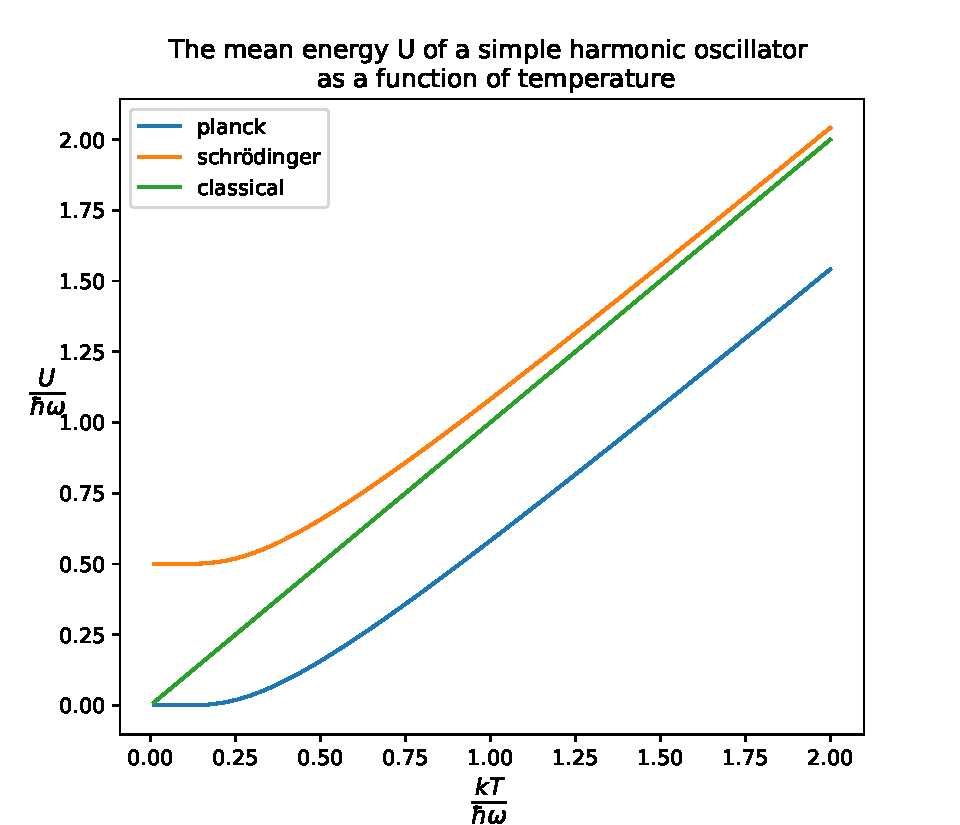
\includegraphics[width=0.6\textwidth]{oscillator_energy.pdf}
    \end{center}
\end{frame}
\end{document}
